\documentclass{article}

\usepackage[a4paper,margin=3cm,headsep=1cm]{geometry}
\usepackage[utf8]{inputenc}
\usepackage{%
    amsmath,
    booktabs,
    fancyhdr,
    pgfgantt,
    titlesec,
    clrscode3e,
    exercise,
    tikz,
    subcaption
}

\tikzstyle{vertex} = [draw, circle, minimum size=0.5cm,fill=lightgray!50!white]

\pagestyle{fancy}

\rhead{Algorithms and Data Structures, S25}
\lhead{Exercises part 1, Lecture 07}
\rfoot{Aalborg University, Copenhagen}
\lfoot{Andreas Holck Høeg-Petersen}

\begin{document}
\thispagestyle{fancy}

\begin{Exercise}[title={Simple training exercises}]
    \Question
    Give an adjacency-list representation for a complete binary tree on 7
    vertices. Give an equivalent adjacency-matrix representation. Assume that
    the edges are undirected and that the vertices are numbered from 1 to 7 as
    in a binary heap. (CLRS 20.1-2)

    \Question
    Show the $d$ and $\pi$ values that result from running breadth-first search
    on the directed graph of Figure 20.2(a), using vertex $3$ as the source.
    (CLRS 20.2-1)

    \Question
    Show the $d$ and $\pi$ values that result from running breadth-first search
    on the undirected graph of Figure 20.3, using vertex $u$ as the source.
    Assume that neighbours of a vertex are visited in alphabetical order. (CLRS
    20.2-2)

\end{Exercise}

\begin{Exercise}[title={Question from Re-exam 2024}]
    \noindent
    Consider the following undirected graph $G$:

    \begin{center}
        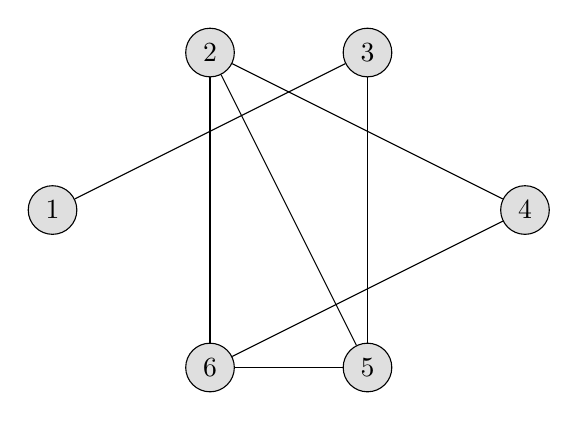
\begin{tikzpicture}
            \node[vertex]   (1)     at (-3,  -2)     {1};
            \node[vertex]   (2)     at (-1,   0)     {2};
            \node[vertex]   (3)     at ( 1,   0)     {3};
            \node[vertex]   (4)     at ( 3,  -2)     {4};
            \node[vertex]   (5)     at ( 1,  -4)     {5};
            \node[vertex]   (6)     at (-1,  -4)     {6};

            \draw (1) -- (3);
            \draw (2) -- (4);
            \draw (2) -- (5);
            \draw (2) -- (6);
            \draw (3) -- (5);
            \draw (4) -- (6);
            \draw (5) -- (6);
        \end{tikzpicture}
    \end{center}

    \Question
    Show the adjacency list representation of the graph (sort the adjacency
    lists by the value in the node).

    \Question
    Use \proc{BFS} (CLRS 4th edition Chapter 20.2, CLRS 3rd edition Chapter
    22.2) on $G$ with node 1 as source (ie.  \proc{BFS}($G$, 1)) and show the
    graph after exactly 4 iterations of the \textbf{while}-loop on line 10. That
    is, annotate each node with the distance found and color each node
    appropriately (either white, gray or black).


    
\end{Exercise}

\begin{Exercise}[title={Fun creative exercises!}]
    \Question
    What is the running time of BFS if we represent its input graph by an
    adjacency matrix and modify the algorithm to handle this form of input?
    (CLRS 20.2-4)

    \Question
    Argue that in a breadth-first search, the value $\attrib{u}{d}$ assigned to
    a vertex $u$ is independent of the order in which the vertices appear in
    each adjacency list. Using Figure 20.3 as an example, show that the
    breadth-first tree computed by BFS can depend on the ordering within
    adjacency lists. (CLRS 20.2-5)

    \Question
    Rewrite the procedure $\proc{DFS}$, using a stack to eliminate recursion.
    (CLRS 20.3-6)
\end{Exercise}


\end{document}

